\documentclass{beamer}
\usetheme{metropolis}

\setbeamertemplate{bibliography item}[text]

\usepackage{amsmath}
\usepackage{amsfonts}
\usepackage{graphicx}
\usepackage{graphics}
\usepackage{setspace}
\usepackage{braket}
\usepackage{float}
\usepackage{nicematrix}
\usepackage{tikz}
\usetikzlibrary{fit}


\makeatletter
\newcommand\mathcircled[1]{%
  \mathpalette\@mathcircled{#1}%
}
\newcommand\@mathcircled[2]{%
  \tikz[baseline=(math.base), color=red] \node[draw,circle,inner sep=1pt] (math) {$\m@th#1#2$};%
}
\makeatother

\newcommand\scalemath[2]{\scalebox{#1}{\mbox{\ensuremath{\displaystyle #2}}}}

\title{Quantum Bogosort}
\subtitle{Systems Software/Algorithms}
\date{May 7, 2022}
\author{George Huebner (Grade 12), Michael Caines (Teacher Sponsor)}
\institute{Walter Payton College Prep, Chicago IL, United States}
\begin{document}
  \begin{frame}
    \maketitle
    \begin{tikzpicture}[overlay, remember picture]
     \node[xshift=-1cm,yshift=-0.33cm, draw=blue] at (current page.north east) {SOFT055};
     \end{tikzpicture}
  \end{frame}
  
  % we looove red tape
  %\begin{frame}[plain, noframenumbering]{Attachments}
    %\begin{columns}
        %\column{0.5\textwidth}
            %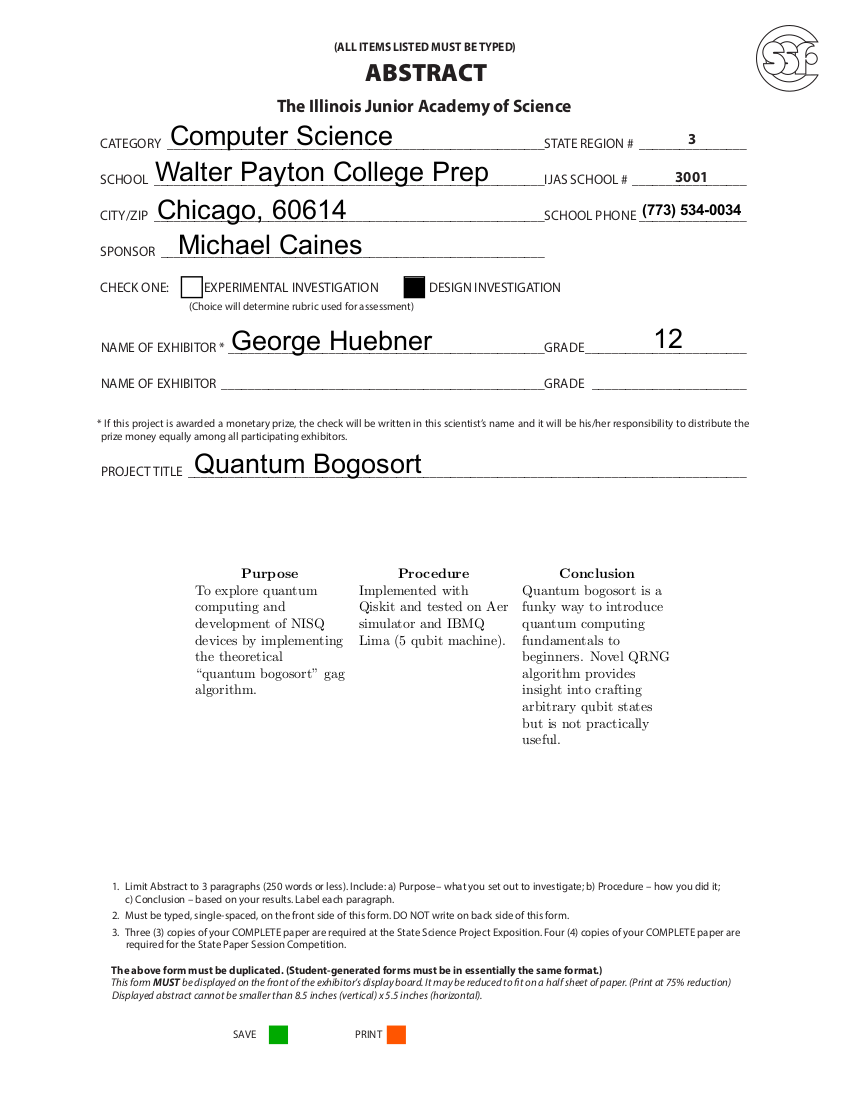
\includegraphics[width=\linewidth]{images/abstract.png}
        %\column{0.5\textwidth}
            %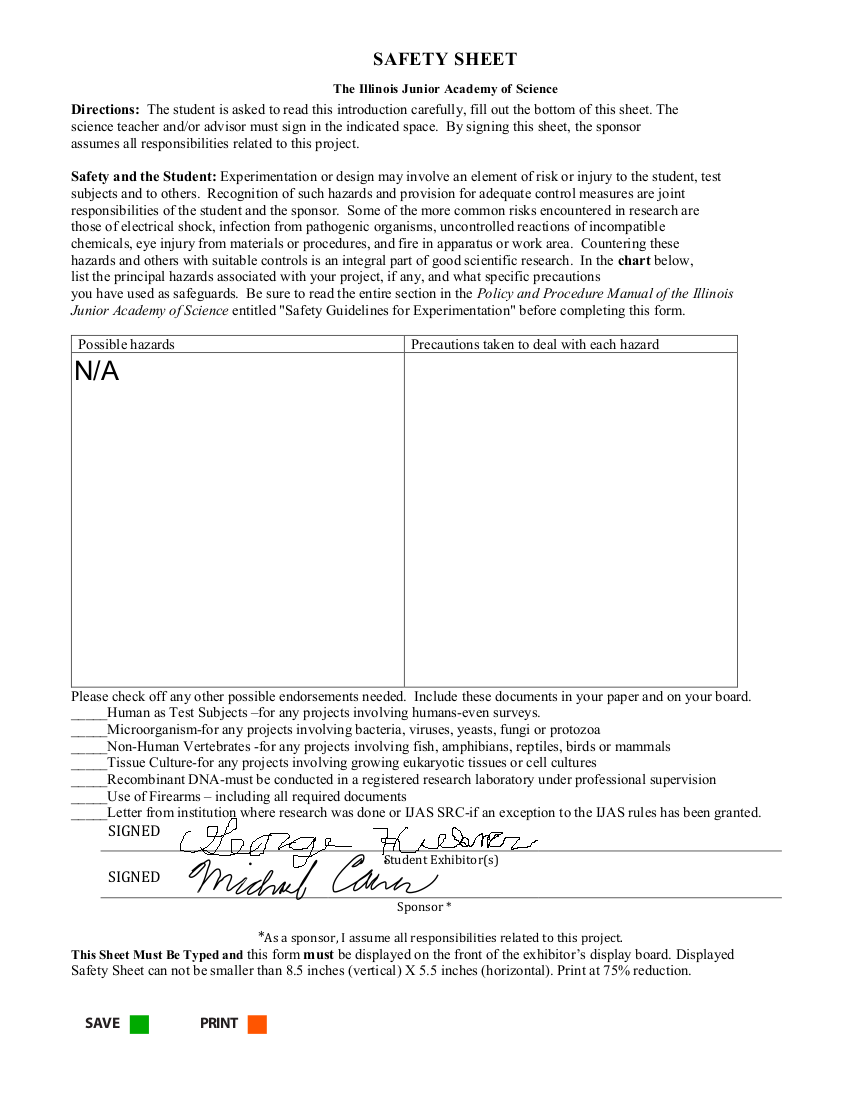
\includegraphics[width=\linewidth]{images/safety_sheet.png}
    %\end{columns}
  %\end{frame}
  
  %\section{Introduction}
  
  %\begin{frame}{Abstract}
    %Gag algorithms are a staple of computer science and provide many a good chuckle. Take, for instance, MiracleSort\textsuperscript{\color{blue}\cite{thompson_2013}}, an algorithm that relies on alpha particle emission to cause erroneous bit flips to sort the list:
    %\begin{center} \texttt{while isSorted(unsorted\_list) is False: \\ \hspace{-70} time.sleep(1000)} \end{center}
    %Despite their apparent uselessness, joke algorithms provide valuable insight into algorithm design and complexity\textsuperscript{\color{blue}\cite{gruber_holzer_ruepp_2007}}. In this paper we propose an implementation to Quantum Bogosort, one such joke algorithm.
  %\end{frame}
  
  %ISEF
  \begin{frame}{Introduction}
      Quantum computing is at a critical junction where hardware has finally caught up to decades of theory, which has sparked renewed interest in the technology. However, the quantum mechanics which make quantum computers fast also make them difficult to learn how to program.
      Training the quantum workforce is essential as demand quickly begins to outstrip the throughput of graduate laboratories. \\
      To meet this need, we propose a quantum algorithm to spark interest in quantum and bridge the understanding between classical and quantum paradigms: \textbf{Quantum bogosort}. \\
      In the same way that in-jokes like the esoteric programming language ``Ook!" can teach programming concepts, quantum bogosort aims to teach quantum computing fundamentals like superposition and entanglement to beginners while being more accessible than traditional textbooks\textsuperscript{\color{blue}\cite{nielsen_chuang_2021}}.
      %Its applied and absurd nature make it more engaging than a traditional textbook, %much like an esoteric language (e.g. BrainF**k) can be more interesting than  programming language design
      %It aims to be more accessible than texts like Chuang's \textit{Quantum Computation and Quantum Information} and more 
  \end{frame}
  
  \begin{frame}{What is Quantum Bogosort?}
    \textit{Classical} Bogosort\textsuperscript{\color{blue}\cite{gruber_holzer_ruepp_2007}} is a (bad) sorting algorithm.
    \begin{enumerate}
        \item Randomly permute the list.
        \item If the list is sorted, done! Otherwise go to step 1.
    \end{enumerate}
    %This has unbounded worst-case time complexity and an expected time complexity of $O(n \cdot n!)$. \\
    \vspace{10}
    \textit{Quantum} Bogosort\textsuperscript{\color{blue}\cite{the_other_tree_2009}} was a proposed extension to bogosort where all list permutations would be placed in superposition. With the `many worlds' interpretation of quantum mechanics, any universe not containing the sorted list would be destroyed (this is where the joke departs from reality). Using the more popular Copenhagen interpretation, our quantum algorithm acts like a random number generator, selecting one permutation of the list at a time; we chose the latter approach and implemented a novel quantum random number generator (QRNG).
  \end{frame}
  
  %\begin{frame}{Attachments}
  %Code + Paper: \href{https://github.com/Borris-the-real-OG/Quantum_Bogosort}{\color{blue} %\underline{github.com/Borris-the-real-OG/Quantum\_Bogosort}}
  %\end{frame}
  
  %\begin{frame}{Acknowledgements}
  %\begin{itemize}
  %\item \href{https://qiskit.org/}{\color{blue} \underline{Qiskit}}
  %\item \emph{We acknowledge the use of IBM Quantum services for this work. The views expressed are those of the authors, and do not reflect the official policy or position of IBM or the IBM Quantum team.\textsuperscript{\color{blue}\cite{ibm_21}}}
  %\item All code was written and tested with Qiskit 0.32.0 \& Python 3.8 on WSL2 Ubuntu 20.04.1.
  %\item Special thanks to Joe Clapis
  %\end{itemize}
  %\end{frame}
  
  %\begin{frame}{Purpose}
  %Just like its classical counterpart, Quantum Bogosort is pretty useless. In fact, classical sorting algorithms have been proven to have a lower bound time complexity of $ \Omega (N \log_2 N) $: there's nothing to optimize! \\
  %\textbf{\textit{However}}, QBS presents a good case study for quantum algorithms; we present an analysis of implementation and complexity of QBS in a similar vein to Gruber et al.'s\textsuperscript{\color{blue}\cite{gruber_holzer_ruepp_2007}} analysis of classic bogosort.
  %\end{frame}
  
  %\section{Algorithm Design}
  
  \begin{frame}{QRNG}
    \begin{columns}[T,onlytextwidth]
        \column{0.58\textwidth}
            \vspace{20}
            Desired State: \\
            $$ \sum_{x=0}^{N-1} \frac{1}{\sqrt{N}} \ket{x_{BE}} $$
            We want an even probability ($\frac{1}{N}$) of measuring any integers from 0 to $N-1$. \\
            \vspace{1em}
            Other QRNGs can only generate even superpositions that are powers of 2; our novel QRNG can generate \textit{any} evenly balanced superposition by `chunking' the problem into smaller subproblems.
            %This is quite easy to do with powers of 2; we just need to use Hadamard gates with control qubits to chunk a big number into smaller subproblems.
       \column{0.4\textwidth}
           `Chunking' 0 to 7
           \begin{align*}
                & \ket{\psi} = \mathcircled{\color{black} \frac{1}{\sqrt{2}}} \ket{0000} + \frac{1}{\sqrt{2}} \ket{1000} \\
                & \mathbf{CH(\psi_0, \psi_{[1, 3]}), \ X(\psi_0)} \\
                & \ket{\psi} = \mathcircled{\color{black} \frac{1}{\sqrt{16}}}(\ket{0000} + \ket{0001} + \\ 
                & ... + \ket{0111}) + \frac{1}{\sqrt{2}} \ket{1000}
            \end{align*}
            \color{red} We mostly care about amplitude as opposed to register state
    \end{columns}
  \end{frame}
  
  \begin{frame}{QRNG}
    \textbf{Limitation:} Hadamard gates create the state $ \frac{1}{\sqrt{2}} \ket{0} + \frac{1}{\sqrt{2}} \ket{1} $. What about states that aren't powers of 2? \\ \\
    \textbf{Solution:} Arbitrary rotation gates allow for qubit superposition with arbitrary amplitudes.
    %Hadamard is just a rotation of $ \frac{\pi}{2} $ around the Pauli Y-axis!
    \begin{align*}
        &\ket{\psi} = \ket{0} \\
        & \text{R}_{\text{y}}(\theta) \ket{\psi} = \begin{bmatrix} \cos \frac{\theta}{2} & -\sin \frac{\theta}{2} \\ \sin \frac{\theta}{2} & \cos \frac{\theta}{2} \end{bmatrix} \ket{\psi} = %-\sin \frac{\theta}{2} \ket{0} + \cos \frac{\theta}{2} \ket{1}
        \cos \frac{\theta}{2} \ket{0} + \sin \frac{\theta}{2} \ket{1}
    \end{align*}
    \textit{Everything in this project is measured in Pauli-Z basis, the most common computational basis.}%so we don't worry about phase or imaginary numbers.}
  \end{frame}
  
  \begin{frame}{Algorithm}
  \begin{enumerate}
      \item If `parts' $= 2^\texttt{len(register)}$, use the control register to apply multi-controlled Hadamard gates to the rest of the register. Done.
      \item If `parts' $\leq 2^\texttt{len(register)}-1$, add \texttt{register[0]} to the control register and skip to step 5.
      \item Calculate $\theta$, R\textsubscript{y}$(\theta)$ the first register qubit, and add it to the control register.
      \item Using the control register, apply multi-controlled Hadamard gates to the rest of the register.
      \item Recurse on the remaining qubits. \\
  \end{enumerate}
  \end{frame}
  
  \begin{frame}{Worked Example}
    \begin{columns}
        \column{0.5\textwidth}
        $$i = 77, \ \ket{\psi} = \ket{0000000}$$
        \column{0.5\textwidth}
        $$\color{blue}\theta_0\color{black} = 2\arccos \sqrt{\frac{77-\color{violet}64}{77}}$$
        \color{violet} Most Significant Bit in register
    \end{columns}
    \begin{align*}
      &\text{R}_y(\color{blue}\theta_0\color{black}, \psi_0), \color{lightgray}\overbrace{\text{X}(\psi_0)}^{\text{Optimized}}\color{black}, \text{CH}(\psi_0, \psi_{[1,6]}), \ \text{X}(\psi_0) = \\
      &\color{green} \frac{1}{\sqrt{77}} (\ket{0000000} + \ket{0000001} + ... + \ket{0111111}) \color{black} + \color{red} \sqrt{\frac{13}{77}} \ket{1000000}
      \end{align*}
      \hspace{60} \color{green} Done with this part \hspace{70} \color{red} New subproblem
  \end{frame}
  
  %\section{Practicality Assessment/Analysis}
  
  \begin{frame}{Generated Circuit}
    \begin{figure}
        \centering
        \begin{tikzpicture}[lablum/.style 2 args={label=below:#1 #2,name=img-#1},
        marr/.style={line width=1mm,-latex}]
         \matrix[column sep=1cm,row sep=5mm] (mat)
         { \node[lablum={1}{Conceptual Circuit\textsuperscript{\color{blue}\cite{chuang}}}]{\includegraphics[width=0.8\textwidth]{images/circuits/conceptual_circuit.pdf}};\\ \\
         \node[lablum={2}{Compiled to Aer Simulator}]{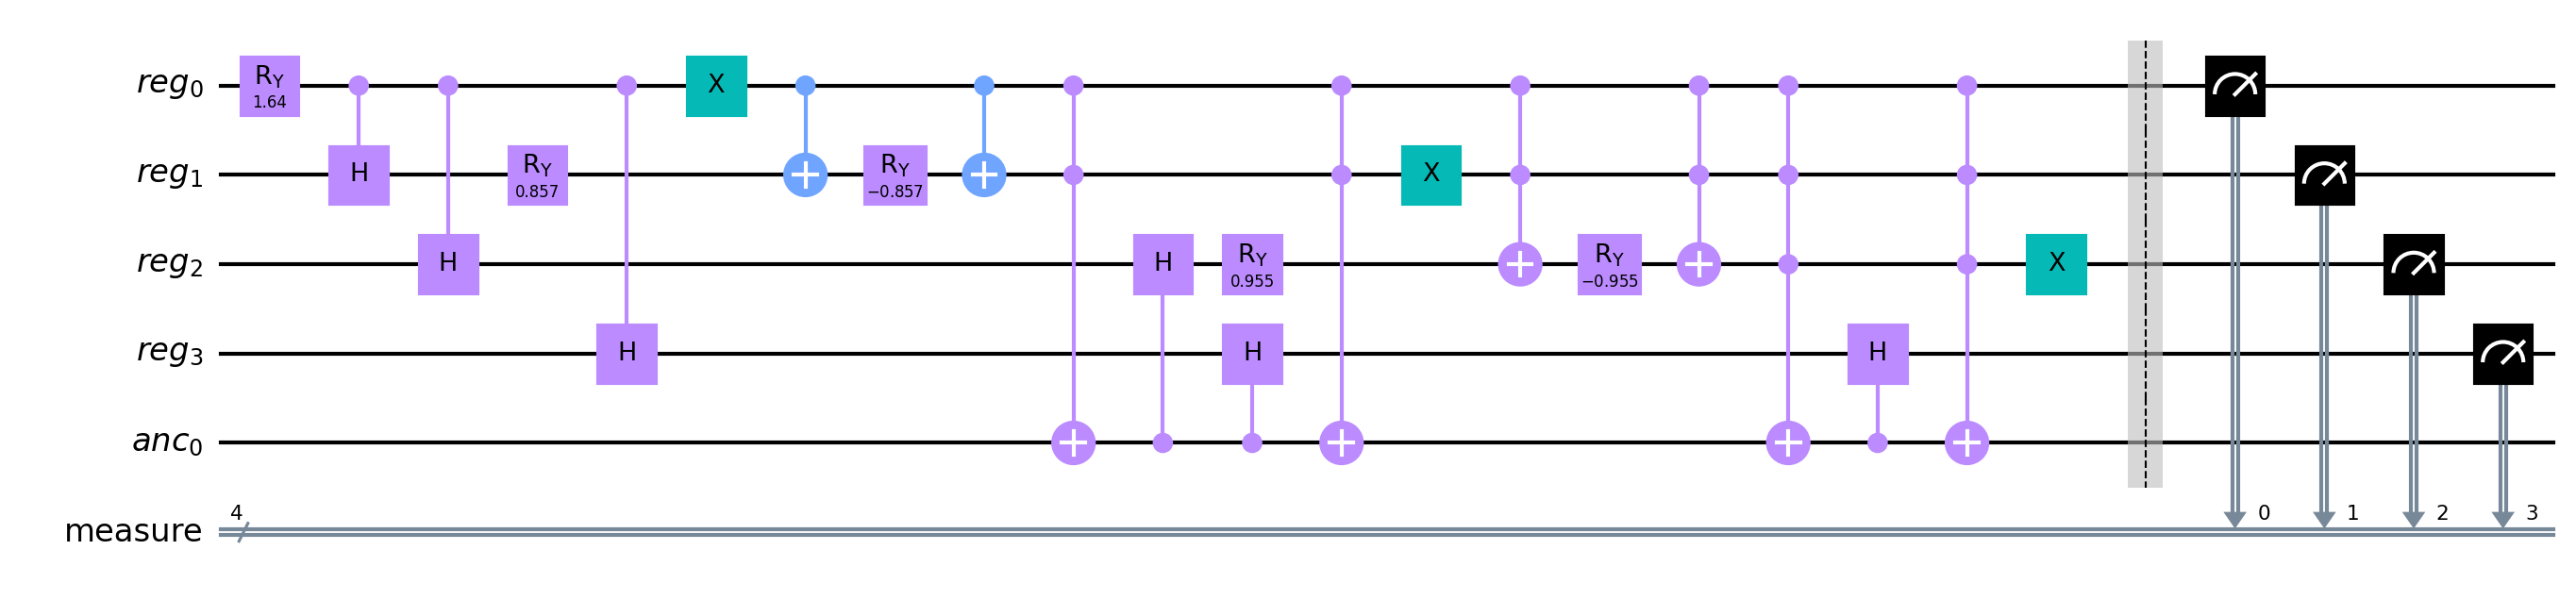
\includegraphics[width=0.8\textwidth]{images/example_circuit.png}};\\};
         \draw[marr] ([yshift=-7mm]img-1.south) coordinate (aux) 
         -- (img-2.north-|aux);
        \end{tikzpicture}
    \end{figure}
   \end{frame}
   
   \begin{frame}{Results}
       \begin{columns}
           \column{0.48\textwidth}
           \begin{center}
           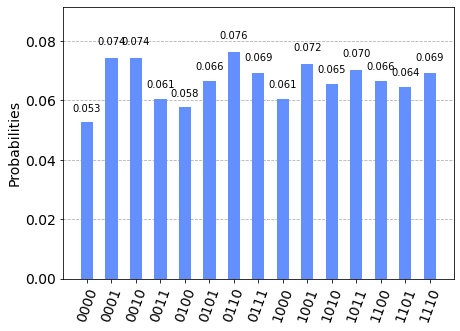
\includegraphics[width=\linewidth]{images/example_measurement.png}
           \textit{Example measurement with } $N = 15$. \\%\texttt{parts = 15}. \\
           \end{center}
           \textbf{Complexity} \\
           $n =$ \# elements \\
           $o =$ \texttt{bin(n).count(`1')} \\
           Many-worlds: $O(o)$ \\
           Copenhagen: $O(o \cdot n!)$
           
           \column{0.48\textwidth}
           Gate count scales with the number of ones in $N$'s binary representation, \textit{\textbf{not}} $N$ itself.
           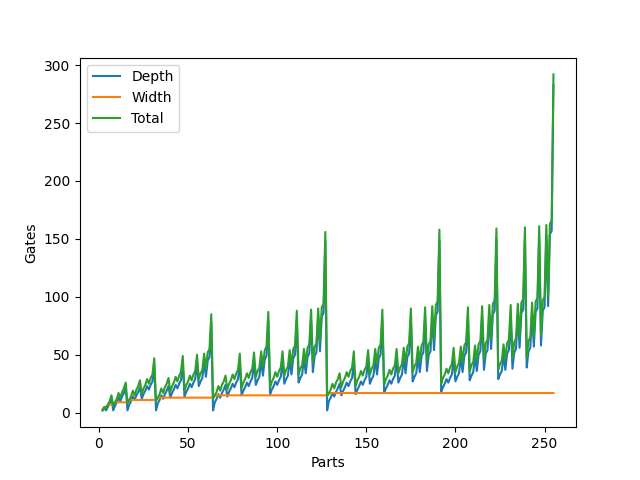
\includegraphics[width=\linewidth]{images/resources.png}
           \textit{Circuit depth, width, and total gate count in relation to} $N$.
       \end{columns}
   \end{frame}
   
   \begin{frame}{Addressing Error}
    \begin{columns}
       \column{0.4\textwidth}
       \small \null \\
       \vspace{10pt}
        Why don't we use $\chi^2$ to check our results? We can calculate the evolution of a qubit's state through statevectors or density matrices (e.g. $\rho$) to prove the probability amplitudes are correct. \\
       \textbf{However}, today's quantum computers are noisy --- real hardware doesn't perform under these ideal conditions. $\rho'$ shows how the state purity changes once the circuit is transpiled with error added to the gates.
       \column{0.6\textwidth}
       \begin{split*}
       &\rho = \underbrace{
       \begin{bNiceArray}{>{\strut}ccccc}[margin,extra-margin = 1pt]
        \frac{1}{15} & \frac{1}{15} & \cdots & \frac{1}{15} & 0 \\
        \frac{1}{15} & \frac{1}{15} & \cdots & \frac{1}{15} & 0 \\
        \vdots & \vdots & \ddots & \vdots & \vdots \\
        \frac{1}{15} & \frac{1}{15} & \cdots & \frac{1}{15} & 0 \\
        0 & 0 & \cdots & 0 & 0 \\
        \CodeAfter
        \begin{tikzpicture}
         \node [draw=red, rounded corners=6pt, inner ysep = 1pt,
            rotate fit=-39, fit = (1-1) (5-5) ] {} ;
        \end{tikzpicture}
       \end{bNiceArray}}_{16 \times 16, \ \color{red}\text{Purity} \ = \ 1} \\[10pt]
       &\rho' = \underbrace{
       \scalemath{0.35}{
       \begin{bNiceArray}{>{\strut}ccccc}[margin,extra-margin = 1pt]
        0.06997 & 0.04275 - 0.00057i & \cdots & 0.0376 + 0.00028i & 0.00036 + 0.00024i  \\
        0.04275 + 0.00057i & 0.06646 & \cdots & 0.03687 + 0.00025i & 0.00002 + 0.0001i  \\
        \vdots & \vdots & \ddots & \vdots & \vdots \\
        0.0376 - 0.00028i & 0.03687 - 0.00025i & \cdots & 0.06272 & 0.00217 + 0.00045i  \\
        0.00036 - 0.00024i & 0.00002 - 0.0001i & \cdots & 0.00217 - 0.00045i & 0.01268  \\
        \CodeAfter
        \begin{tikzpicture}
         \node [draw=red!50, rounded corners=4pt, inner ysep = -1pt,
            rotate fit=-11, fit = (1-1) (5-5) ] {} ;
        \end{tikzpicture}
       \end{bNiceArray}
       }}_{16 \times 16, \ \color{red}\text{Purity} \ = \ 0.42118 \\}
       \end{split*}
       \tiny \centering \textit{Using noise model from IBMQ\textsuperscript{\color{blue}\cite{ibm_21}} Santiago. Note that this does not take into account measurement, reset, relaxation or decoherence errors.} % It could, but I'm lazy. ¯\_(ツ)_/¯
   \end{columns}
  \end{frame}
  
  \begin{frame}{Conclusion}
  %Quantum Bogosort is not a practical algorithm, but it's helpful in teaching quantum computing fundamentals in a fun way. \\
  Although potetially infeasible due to its ballooning gate count, the QRNG algorithm could be repurposed for state preparation in tandem with other quantum algorithms. However, it's not necessarily the \textit{fastest} way for state preparation; transpilation optimizations and optimal gate decompositions pose interesting extensions to this problem that are especially pertinent with current quantum computers. Additionally, it could be interesting to further design around the constraints of NISQ devices by executing QRNG incrementally in order to reduce decoherence and relaxation errors. \\%Although this is one way to achieve even measurement amplitudes over a register, it's not necessarily the \textit{fastest} way; transpilation optimizations and optimal gate decompositions pose interesting extensions to this problem that are especially pertinent with current quantum computers.  \\
  %There are dozens of error mitigation schemes for quantum computers, however implementing robustness was not a focus of this project. For example, by trying to optimize around the abysmal $ O(\log_2 n!) $ space complexity via `dividing and conquering', we end up implementing quicksort! %Quantum Bogosort doesn't provide a quantum advantage over its classical counterpart (except by being truly random)
  \vspace{0.5em}
  Although we successfully implemented quantum bogosort and made certain quantum computing concepts more accessible, this algorithm did not cover interference/phase --- important, fundamental ideas that are present throughout most of quantum computing. 
  \end{frame}
  
  \begin{frame}{Bibliography}
  \bibliographystyle{ieeetr}
  \bibliography{sources}
  \end{frame}
  
  
\end{document}
